\subsection{Coupling between components}
    According to the definition
    \footnote{Coupling definition: \cb{
    \url{https://en.wikipedia.org/wiki/Coupling\_(computer\_programming)}}}:
    \begin{adjustwidth}{1.5cm}{}
        \textit{Coupling is the degree of interdependence between software modules; a measure of how closely connected two routines or modules are; the strength of the relationships between modules.}\\
    \end{adjustwidth}
    Tight coupling in a software system can be associated with more interdependency between components, more coordination and more information flow; on the other hand, low coupling can be associated with less interdependency, coordination and information flow. \\
    Tightly coupled systems can have the following characteristics, often seen as disadvantages:
    \begin{enumerate}
        \item A change in one module can cause a ripple effect of changes in other modules 
        \item Assembly of modules will take considerably longer time thanks to the increased interdependency between them and the high flow of information
        \item Using a single module as a standalone might be difficult due to other modules also being needed.
    \end{enumerate}
    Looking at these characteristics, we can motivate the general idea that good design usually is related to loose coupling in the system.\\\\
    In order to analyze the design quality of the system, we have to analyze the coupling between its components. As such, we will make use of two metrics, namely \texttt{FANIN} and \texttt{FANOUT}. These two metrics were borrowed from logic circuit design, and they represent the number of occurrences of a class (how many times a class is being called) and the number of classes a certain class calls in its definition. They can be used to indicate the extent to which a component is independent, as well as how much responsibility it has. Ideally, in a low coupled system, these two metrics should be as low as possible. 
    \\\\
    When describing packages, we can talk about two types of coupling:
    \begin{enumerate}
        \item \textbf{Afferent coupling AC}\\
        The number of packages that depend upon classes in a certain package. It indicates the package's responsibility.
        \item \textbf{Efferent coupling EC}\\
        The number of packages that the classes in a package depend upon. It indicates the package's independence.
    \end{enumerate}
    The following section will document our findings of the FANIN and FANOUT metrics on the \cb{optaplanner-core} package.
    
    \begin{itemize}
        \item The \cb{api} folder\\
        Looking at the metrics that Designite found for this folder, we found that there are two classes with a very high FANIN value: 149 and 147 - which means that there are as many classes that make use of each of them. The high FANIN value implies a very high dependence of the system on these classes, making them potential candidates for the "God element" code smell. Both of the classes have the \cb{score} as concern, and this is expected since the system's main functionality revolves around the score of the algorithms. Not only that, but 6 out of the 10 classes with the highest FANIN values are in the same package: \cb{api.score}. An overview of the 10 highest FANIN values can be seen in Figure \ref{fig:faninapi}.
        \begin{figure}[H]
            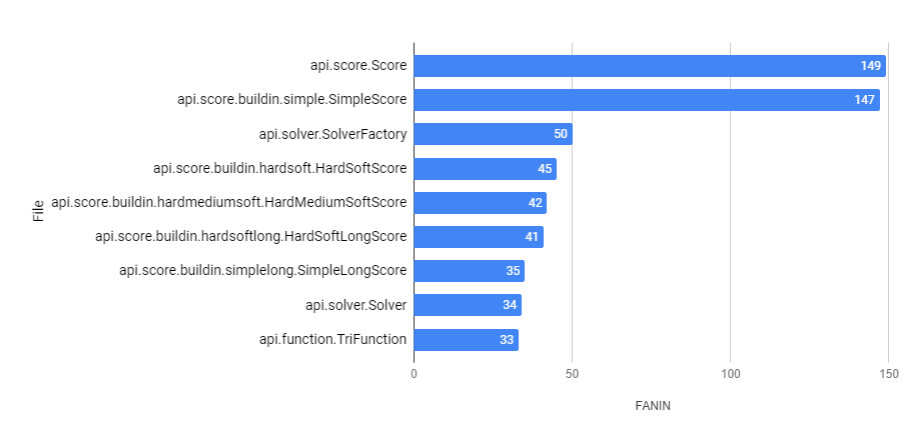
\includegraphics[scale=0.8]{figures/step4/step4.2/FANIN_api.PNG}
            \caption{The classes with the highest FANIN value in the \cb{api} folder}
            \label{fig:faninapi}
        \end{figure}
        When analysing the FANOUT value, we have found that in this folder, most of the files with a high FANOUT value are test files for the \cb{score} package, which is again expected considering that this package is very important for the functionality of the system. An overview of the 10 highest FANOUT values can be seen in Figure \ref{fig:fanoutapi}. The highest values were 16 and 15 - but again these can be justified by the fact that in test files, a lot of classes must be instantiated and initialized in order to perform realistic tests. 
        \begin{figure}[H]
            \centering
            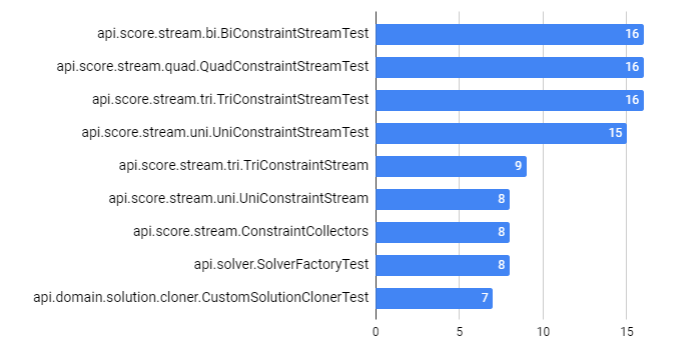
\includegraphics[scale=0.8]{figures/step4/step4.2/FANOUT_api.PNG}
            \caption{The classes with the highest FANOUT value in the \cb{api} folder}
            \label{fig:fanoutapi}
        \end{figure}
        
        
        \item The \cb{config} folder\\
        The most dependable file in this folder is a \cb{utils} file, namely  \cb{config.util.ConfigUtils}. Since such a file contains utility specifications that are useful for the whole system, it is expected that a lot of classes rely on it and use it - in order to avoid duplicate code, and also, to have all the configurations centralised in order to keep maintainability high. \\
        The second most dependable class is a configuration file for the solvers - this can be explained by the fact that the system has a lot of possible \cb{solver} instances that can be used with different configurations. As such, this \cb{SolverConfig} file can be used to keep the configurations centralised. \\
        An overview of the most dependable files (highest FANIN values) can be seen in Figure \ref{fig:faninconfig}
        \begin{figure}[H]
            \centering
            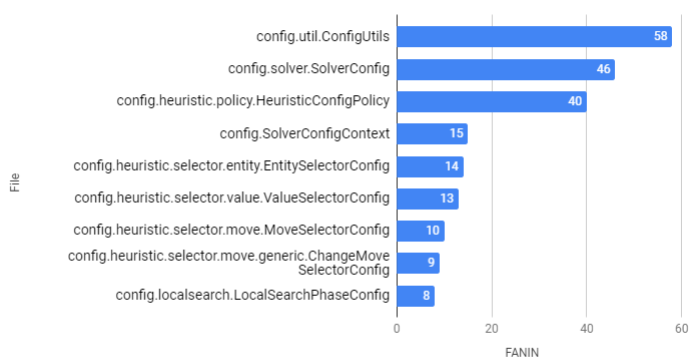
\includegraphics[scale=0.8]{figures/step4/step4.2/FANIN_config.PNG}
            \caption{The classes with the highest FANIN value in the \cb{config} folder}
            \label{fig:faninconfig}
        \end{figure}
        
        FANOUT represents the responsibility of a file, so how many other files it is responsible for. In this folder, the files with the most responsibilities are configuration files for the \cb{Solver} class, or for the classes that are concerned with the configuration of the search algorithms. The high responsibilities of these classes can be due to the fact that their functionalities are the most complex and they require a lot of information in order to set them up correctly.
        An overview of the most dependable files (highest FANOUT values) can be seen in Figure \ref{fig:fanoutconfig}
        \begin{figure}[H]
            \centering
            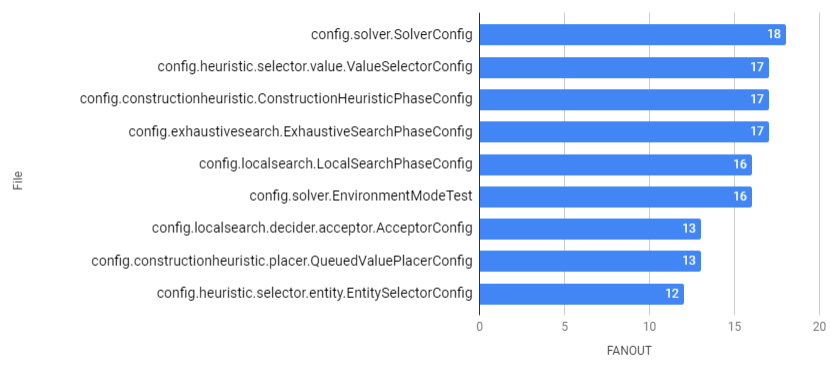
\includegraphics[scale=0.8]{figures/step4/step4.2/FANOUT_config.PNG}
            \caption{The classes with the highest FANOUT value in the \cb{config} folder}
            \label{fig:fanoutconfig}
        \end{figure}
        
        
        \item The \cb{impl} folder\\
        From the previous analyses, we know that this folder is the biggest and most complex. As such, we also expect it to be the most dependable and having a lot of responsibilities. Since there were a lot of classes with a high FANIN value, we have included the top 15 of them in our analysis, as they can be seen in Figure \ref{fig:faninimpl}. The most dependable class has a very high FANIN score, 163. It is also the class that we have previously found as the biggest, in terms of LOC and complexity. It is the \cb{SolutionDescriptor} class, and it is the most dependable file in the whole system. This high dependence on this file can be explained by the fact that the system provides a lot of ways of describing solutions to a lot of different problems, and this file has the classes that are instantiated the most. \\
        The second dependable file is \cb{ScoreDirector}, again a very big, complex file, and it is being used to calculate the scores of the different solutions - which we expect to be the argument for the high dependency value, since this class is oftenly used with the \cb{SolutionDescriptor.} \\
        An overview of the top 15 highest FANIN values can be seen in Figure \ref{fig:faninimpl}.
        \begin{figure}[H]
            \centering
            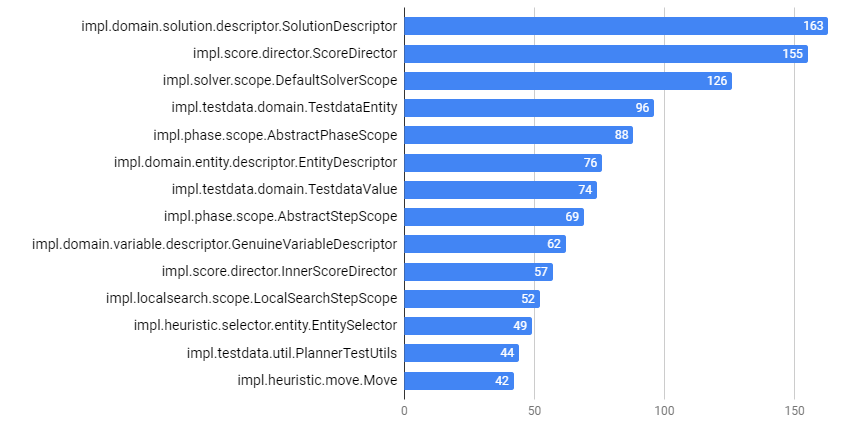
\includegraphics[scale=0.8]{figures/step4/step4.2/FANIN_impl.PNG}
            \caption{The classes with the highest FANIN value in the \cb{impl} folder}
            \label{fig:faninimpl}
        \end{figure}
        \cb{SolutionDescriptor} was found to also be the file with the most responsibility, with a FANOUT value of 34 - meaning that it is responsible for 34 other classes. The arguments are similar to the ones mentioned above. The rest of the files with high FANOUT values in this location are again test classes, or concerned with the score of an algorithm. An overview of the top 10 highest FANOUT values can be seen in Figure \ref{fig:fanoutimpl}.
        \begin{figure}[H]
            \centering
            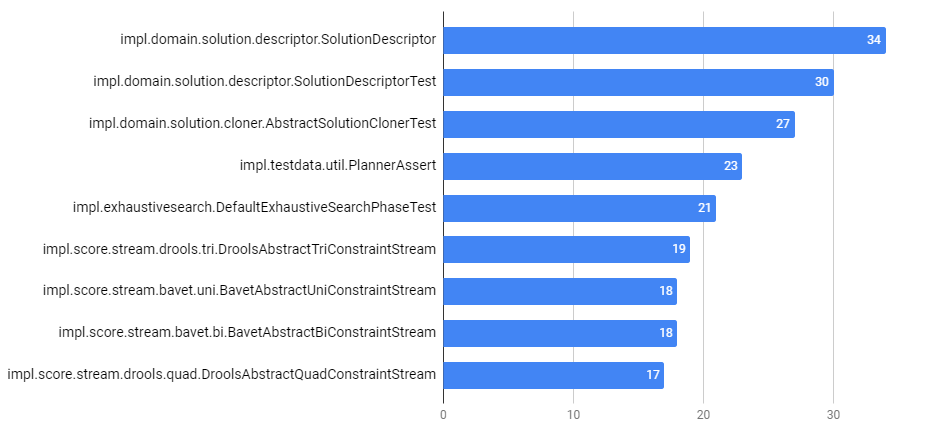
\includegraphics[scale=0.8]{figures/step4/step4.2/FANOUT_impl.PNG}
            \caption{The classes with the highest FANOUT value in the \cb{impl} folder}
            \label{fig:fanoutimpl}
        \end{figure}
    \end{itemize}
